\renewcommand\labelenumi{(\roman{enumi})}
\renewcommand\theenumi\labelenumi

\chapter{Introduction}
\label{chapterIntro}
\chaptermark{Introduction}

Explicar el problema al qual ens estem adre\c{c}ant 

\textcolor{red}{20-25 PAGINES}

\textcolor{red}{Fer a la intro, despres de quan introdueixo els local markets icons,m quan he dexplicar la contribucio a la tesi. Explicar quin son els tres agents que analitzo, en aquest cas dos, aggregator i DSO. I llavors posar la interaccio entre ells, la flex request, flex forecast i flex activation, posar tots els agents. Llavors a cada chapter indico quina cadena estic treballant, i despres en difuminat indico quina cadena no estic activant.}

\begin{figure}[]
	\centering
	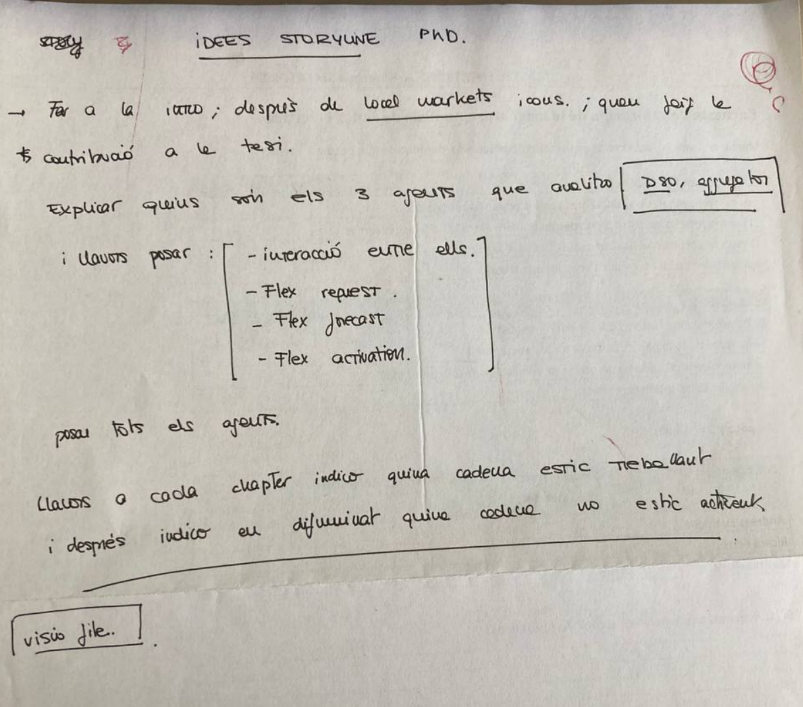
\includegraphics[width=1\columnwidth ]{ChapterIntro/Figures/idea.png}
	   %\vspace*{-8cm}
		\caption{XXXX}  
\end{figure}


\section{Smart grids}

\subsection{Distributed Energy Resources} \label{subsec:DG}

\section{Distribution networks: challenges}

\section{Electricity markets}
incloure aqui capitol del llibre de local and micro power markets? 
Power market fundamentals 


\section{Regulation framework and new agents in the energy transition}
entregable que vam fer amb el pau Plana TFG

\section{Local electricity markets}

\section{Sustainability of smart grids and DERs}
Explicacio sobre que entenem per sostenibilitat. Quina relacio hi ha entre sostenibilitat i smart grids local markets 

\newpage 
\section{Objectives and scope}

\newpage 
\section{Thesis related work and activities}
	

\newpage 
\section{Thesis outline}
	


